%!TEX root = draft.tex
\section{Overview}
\label{sec:overview}

In this section we will firstly describe the system and program model
we assume, and we will then illustrate our main contribution in two
interesting CRDT implementations extracted from~\cite{ShapiroPBZ11}.

\begin{figure}[t]
  % \centering
\begin{lstlisting}[caption={Pseudo-code of the Replicated Growable
Array (RGA) CRDT (adapted from~\cite{ShapiroPBZ11})},
captionpos=b,label={lst:rga}]
  payload Ti-Tree N, Set Tomb
  initial N = @|$\emptyset$|@, Tomb = @|$\emptyset$|@
  //@ initial lin = @|$\epsilon$|@

  addAfter(a,b) :
    atSource :
      precondition : a = @|$\circ$|@ or (a != @|$\circ$|@ and (a,_,_) @|$\in$|@ N and a @|$\not\in$|@ Tomb)
      let ts@|$_{\mathtt{b}}$|@ = getTimestamp()
      //@ let lin = insert(lin, @|$\alabelshort[{\tt addAfter}]{a,b}$|@, ts@|$_{\mathtt{b}}$|@)
    downStream(a, ts@|$_{\mathtt{b}}$|@, b) :
      N = N @|$\cup$|@ {(a, ts@|$_{\mathtt{b}}$|@, b)}
      //@ N@|$'$|@ = N @|$\cup$|@ {(a, ts@|$_{\mathtt{b}}$|@, b)}

  remove(a) :
    atSource :
      precondition : (a,_,_) @|$\in$|@ N and a @|$\notin$|@ Tomb
      //@ let lin = insert(lin, @|$\alabelshort[{\tt remove}]{a}$|@, @|$\mathsf{max}\, \{\tsof(\alabel):\alabel\in \alabelset \}\,$|@)
    downStream(a) :
      Tomb = Tomb @|$\cup$|@ {a}
      //@ Tomb@|$'$|@ = Tomb @|$\cup$|@ {a}

  read() :
    let ret-list = traverse(N, Tomb)
    //@ let lin = insert(lin, @|$\alabellongind[{\tt read}]{}{{\tt ret\text{-}list}}{}$|@, @|$\mathsf{max}\, \{\tsof(\alabel):\alabel\in \alabelset \}\,$|@)
    return ret-list
\end{lstlisting}
\end{figure}
%       precondition: a = @|$\circ$|@ or (a != @|$\circ$|@ and (a, ts@|$_{\mathtt{a}}$|@,_) @|$\in$|@ N)
%       precondition : (a,_,_) @|$\in$|@ N

% \gpnote*[nomargin]{}{
%   Section sketch:
%   \begin{itemize}
%   \item Informal explanation of the system model. Multiple replicas,
%     clients connect to any replica. Operations are propagated lazily.
%   \item Explanation of the program model. We explain the code of RGA
%     (\lstinline|atSource|, \lstinline|downStream|). Conflict
%     resolution. Commutativity.
%   \item We give a first intuition about the \CRDTLin{} of RGA. We
%     might explain why standard Linearizability is not good enough.
%   \item We present OR-Set. We explain that the linearization of OR-Set
%     is more complicated without getting too tangled into de details.
%     OR-Set is important because we need to explain that some
%     operations will see a sub-sequence of the global linearization
%     (in contrast to RGA above).
%   \item If needed we can talk about the compositionality problem.
%   \end{itemize}
% }

\subsection{System Model}
\label{sec:sys-model}

We assume that the system is comprised of multiple nodes in a network.
In this work we will be concerned with the implementation of CRDTs,
and we will usually concentrate our discussion to the behaviors
allowed for \emph{an instance} of the data type.
We will generically call such an instance an \emph{object}.
As mentioned in~\autoref{sec:introduction} we assume that objects are
replicated among the participating nodes of the system -- which we
shall call replicas.

\begin{figure}[t]
  \centering
  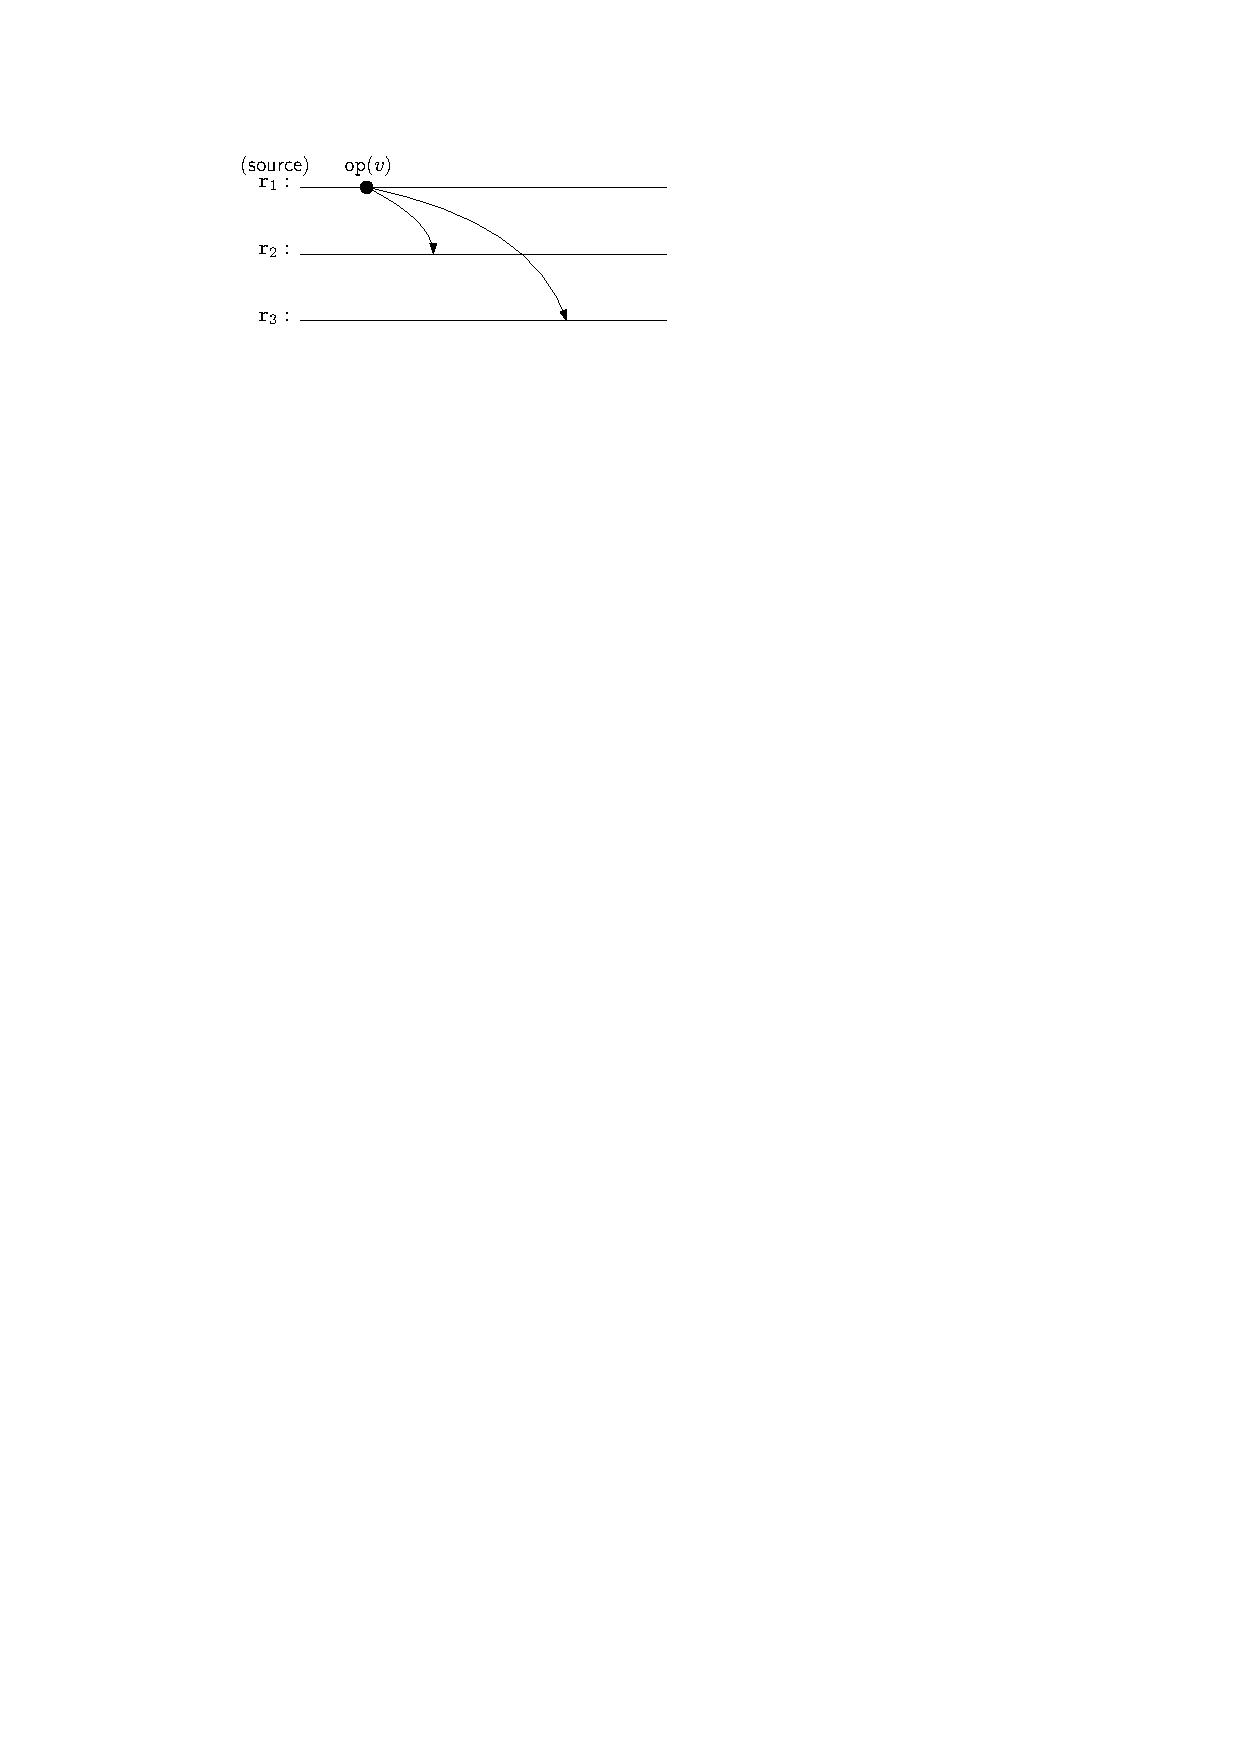
\includegraphics[scale=.4]{figures/sys-mod}
  \caption{CRDT System Model}
  \label{fig:sys-mod}
\end{figure}

The execution model for an operation \lstinline|op(v)| on a replicated
object is depicted in~\autoref{fig:sys-mod} and it proceeds as follows:
\begin{itemize}
\item A client, which is a program issuing calls to the object, connects
  to any one replica (a node of the system holding a copy of the object)
  and performs the operation in that replica, we shall call such a
  replica the origin or \emph{source}. The source of \lstinline|op(v)|
  in~\autoref{fig:sys-mod} is the replica on the top.
\item Then, executing an operation is done in two phases.
  Assuming that the operation requires reading and updating the state
  of the object, the state of the object in the source replica is read
  first.
  We shall sometimes refer to this part of the operation as the
  generator following~\cite{ShapiroPBZ11}.
  Then, if the state needs to be changed as part of the operation --
  e.g. an \lstinline|addRight| operation of RGA -- an update is
  generated which shall be executed in all the replicas holding copies of the
  object.
  We shall refer to the update as the effector.
  We assume throughout this paper that effectors are executed
  immediate in the source replica.
  This is represented by the dot at the source replica
  in~\autoref{fig:sys-mod}.
\item Finally, as the system progresses, the effector of the operation
  will be delivered to each of the replicas holding a copy of the
  object.
  This is represented by the target of the arrows
  in~\autoref{fig:sys-mod}.
\end{itemize}
% This model is depicted in~\autoref{fig:system-model}.
% \fxwarning[nomargin, inline]{We need the picture}.

\paragraph{CRDT implementations}

Following the description above, \citet{ShapiroPBZ11} presents the code
for a number of CRDT implementations.
%
Here we consider the code of the RGA algorithm presented
in~\autoref{lst:rga}.
%
Let us first consider the structure of the data type implementation:
\begin{itemize}
\item The keyword \lstinline|payload| introduces the state that is
  used to represent the object. This is akin to the fields of a class
  file in an object oriented language such as Java. In the specific
  case of RGA we have a variable \lstinline|N| of type
  \lstinline|Ti-Tree| (to be discussed later), and a variable
  \lstinline|Tomb| of type \lstinline|Set|.
\item After that we find the definitions of the three operations we
  discussed in the introduction: \lstinline|addAfter|,
  \lstinline|remove| and \lstinline|read|.
\item The effectful operations \lstinline|addAfter| and
  \lstinline|remove| have two labels marked in red:
  \lstinline|atSource| and \lstinline|downStream|.
  These represent the code to be executed as the generator and
  effector respectively. Hence, the code under the label
  \lstinline|atSource| is executed only at the source replica and it
  generates the arguments that the code under \lstinline|downStream|
  will execute in each of the replicas.
\item We can also notice that under the labels there are
  \lstinline|precondition| annotations indicating facts that are
  assumed about the state of the object upon execution of either of
  the generator or effector of the operation.
\end{itemize}
Reconsidering~\autoref{fig:sys-mod} we can then say that the
source of the arrows in each replica represent the execution of an
\lstinline|atSource| jointly with the \lstinline|downStream| of the
operation at the source replica.
%
The sink of the arrows represents the delivery and execution of the
generator of the operation in a replica other than the source.


In the rest of this section we consider two examples of CRDT
implementations and their linearization arguments.

\subsection{RGA CRDT Implementation}
\label{sec:rga-crdt-impl}

% \paragraph{RGA CRDT implementation}
As it is common to many CRDT implementations, in RGA replicas will use
a timestamp mechanism to keep track of the causality between updates
to the list, effectively capturing when two updates are concurrent,
and moreover, they will keep the information relating the causal order
in which elements are added to the list.
%
Provided with this causality -- or lack thereof-- information, the
timestamps will be used to resolve conflicts in a deterministic way.
%
More concretely, each replica will keep what we shall name a
\emph{Timestamp Tree} (\lstinline|Ti-Tree|) containing in every tree
node a pair with: the element added to the list (for instance the
character \lstinline|b|), and a timestamp associated to it
(\lstinline|t|$_{\mathtt{b}}$) which will be used to resolve
conflicts.
%
We will encode the tree as a set containing triples (corresponding to
nodes) of the form (\lstinline|a|, \lstinline|ts|$_{\mathtt{b}}$, \lstinline|b|)
representing the fact that there is an element \lstinline|b| in the
tree with timestamp \lstinline|ts|$_{\mathtt{b}}$ and whose parent is the item
\lstinline|a| also present in the tree.
%
The tree-ness property will be ensured by construction.


If we look at the \lstinline|atSource| portion of the
\lstinline|addAfter(a,b)| method we can see that precondition requires
the \lstinline|a| to exist in the tree before the insertion of
\lstinline|b| after it.
%
We remark at this point that the data structure is initialized with a
preexisting initial element denoted by $\circ$.
%
The generator then samples a timestamp \lstinline|t|$_{\mathtt{b}}$
for \lstinline|b| which is assumed to be larger than any
timestamp presently occurring in the \lstinline|Ti-Tree|
\lstinline|N|.
\gpnote{Add note about uniqueness of TSs (rid).}
%
Looking at the \lstinline|downStream| portion of
\lstinline|addAfter(a,b)| we see that the effect of the operation is
to add the triple \lstinline|(a, ts|$_{\mathtt{b}}$\lstinline|, b)|
in the replicas own copy of \lstinline|N|.
%
Then, the tree structure is consistent with the causality of
insertions in the data structure.
%
Notice that a client of the object will only ever attempt to add an
element after another element which has already seen (mandated by the
\lstinline|addAfter| API).
%
Hence, the parent node of any node was inserted before it, and is
causally related to it.
%
Similarly, nodes that are not related to each other on any path of
the tree (eg. siblings) are not causally related.\footnote{The converse
  is not true. There can be nodes that are linked by ancestry in the
  tree resulting from concurrent operations, but this does not affect
  the correctness of the algorithm.}
%
An example of such a tree is shown in~\ref{fig:rga-tree}.

Considering a \lstinline|Ti-tree| constructed in this way, we can
obtain a list by traversing the tree in pre-order fashion, with the
proviso that siblings are ordered according to their timestamps.
%
\autoref{fig:rga-tree} shows the tree that results from the given
tree.


\gpnote*{By Chao. Should be elsewhere}{
\figurename~\ref{fig:how RGA works} gives a example of how RGA do conflict resolution for concurrent $addAfter$ operations, and how it do $remove$: if from one local state we do concurrent $\alabelshort[addAfter]{b,c}$ and $\alabelshort[addAfter]{b,d}$, then it converges. If we then do $\alabelshort[remove]{b}$, we just add $b$ into tombstone. Here we assume $\ats_a$, $\ats_b$, $\ats_c$ and $\ats_d$ is the timestamp of $a$, $b$, $c$ and $d$, respectively, and the timestamp order be $\ats_a < \ats_b < \ats_c < \ats_d$.
}

\begin{figure}[t]
  \centering
  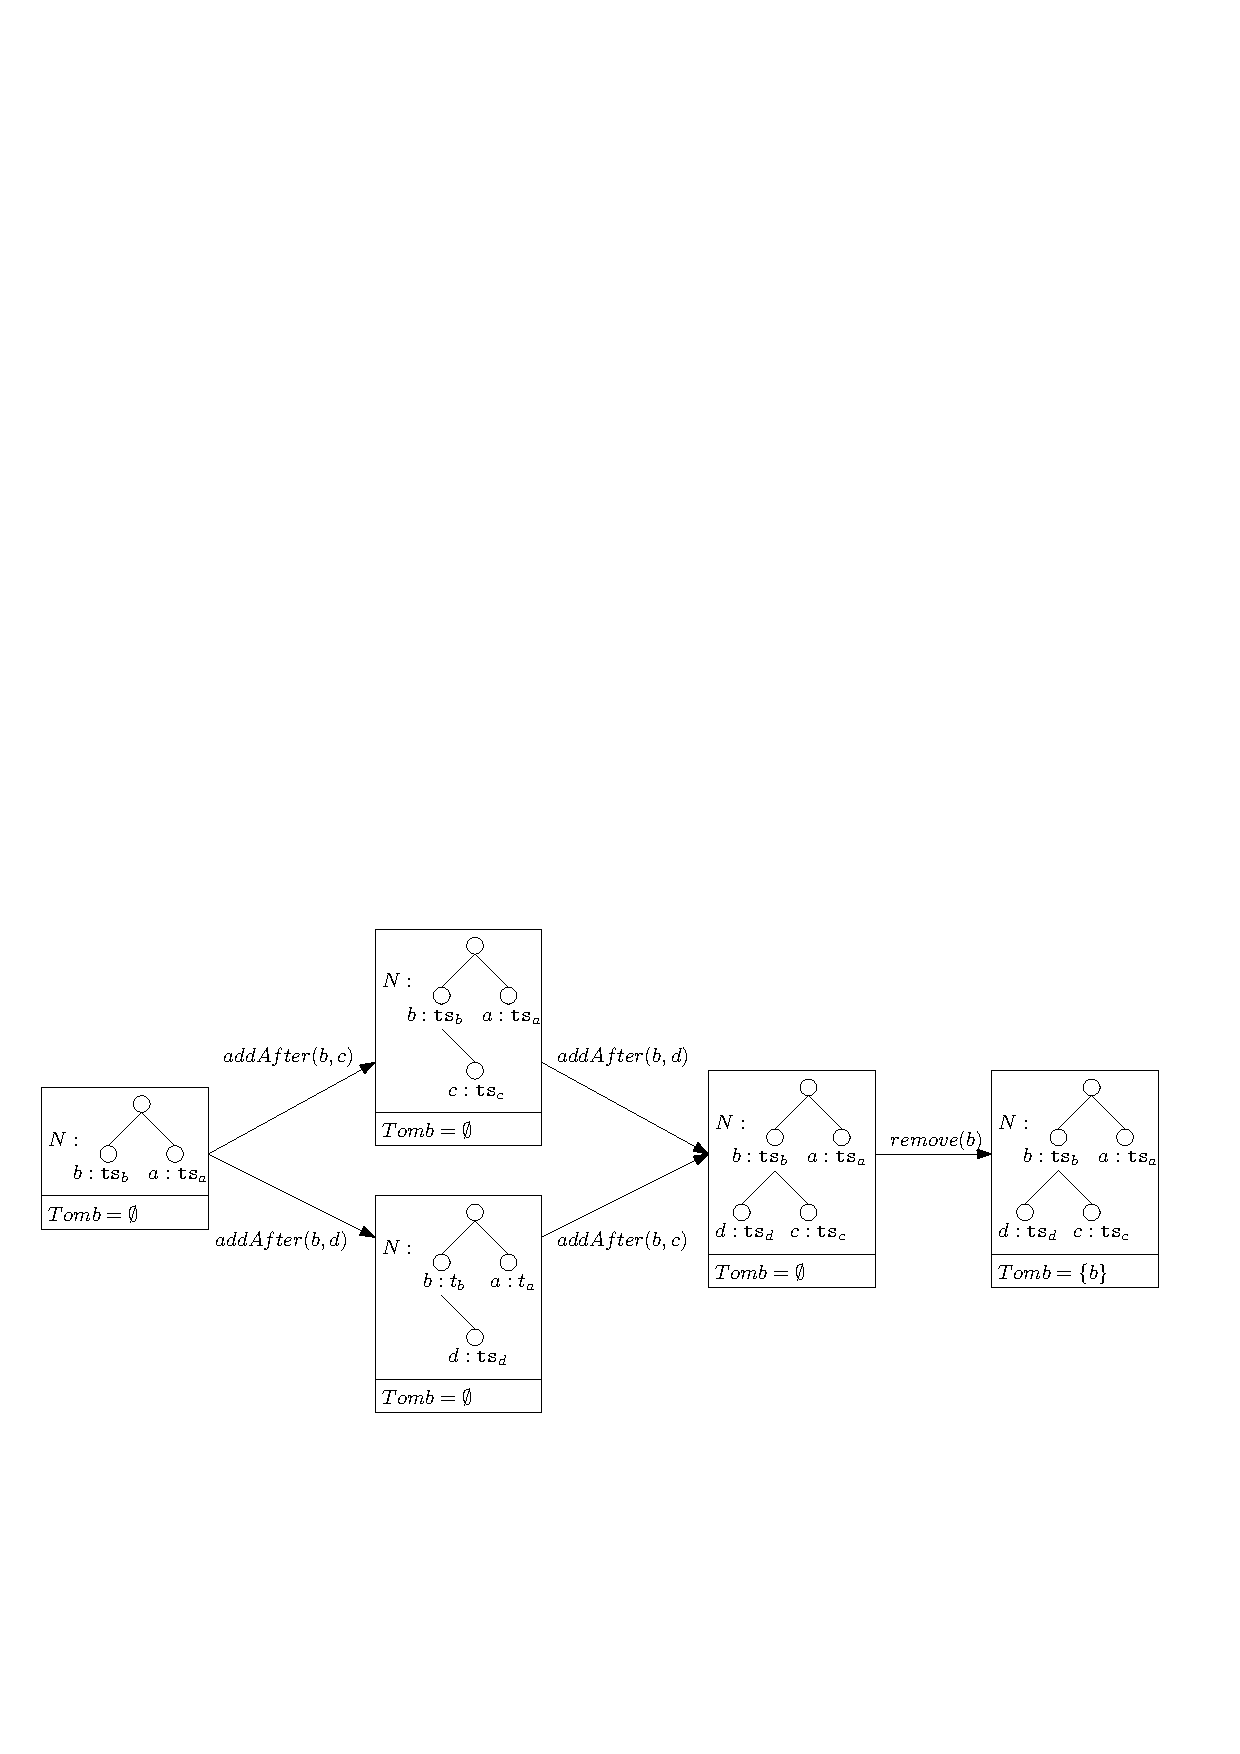
\includegraphics[width=0.85 \textwidth]{figures/HowRGAWork.pdf}
% \vspace{-10pt}
  \caption{An example of conflict resolution of RGA, and how we do remove.}
  \label{fig:how RGA works}
\end{figure}

\begin{figure}[t]
  \centering
  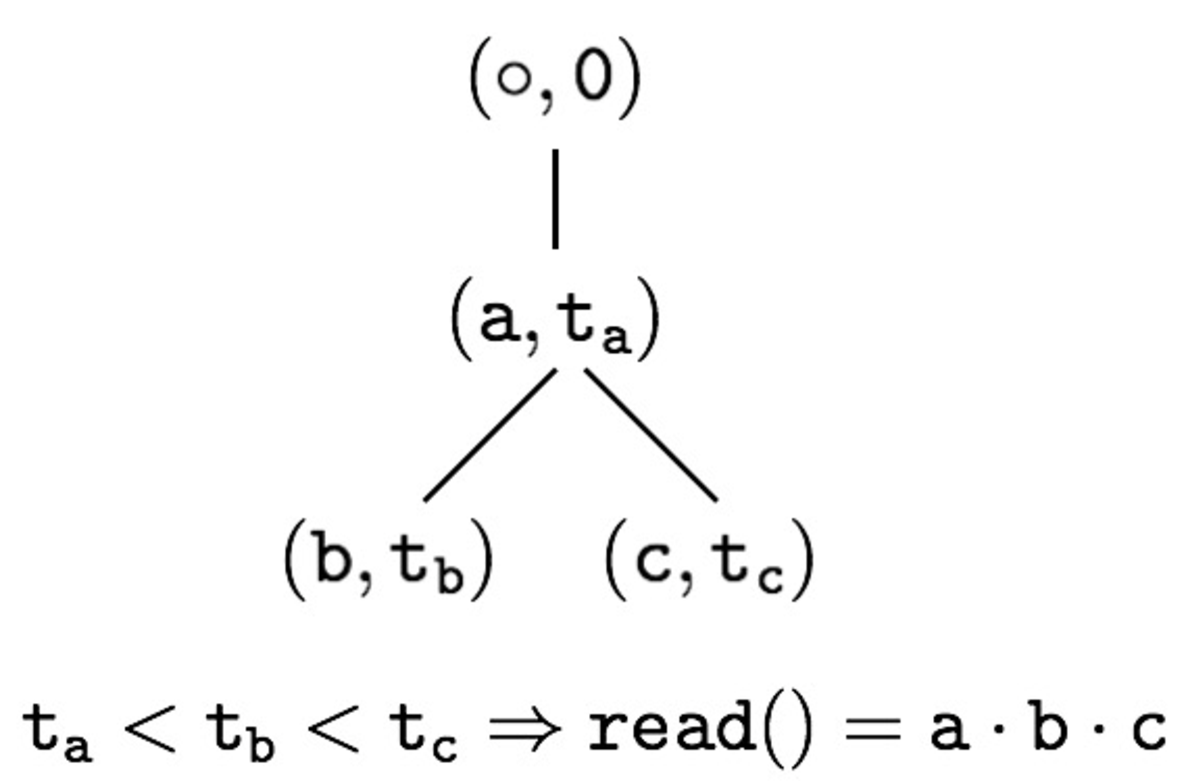
\includegraphics[scale=.25]{figures/simple-ti-tree}
  \caption{RGA Ti-tree example.}
  \label{fig:rga-tree}
\end{figure}


We have so far ignored the \lstinline|remove| operation.
%
Consider the case where a client issues an \lstinline|addAfter(a, b)|
on a replica whereas another client issues a \lstinline|remove(a)|
operation in another replica.
%
If the effector of \lstinline|remove(a)| reaches every replica after
the effector of \lstinline|addAfter(a, b)| there is no problem since
the semantics is obvious (the element \lstinline|a| is removed after
the element \lstinline|b| has been added).
%
However, if the operations reach some replica in the opposite order
(recall that these are concurrent operations) we have a problem, since
the precondition of the effector of \lstinline|addAfter(a, b)|
requires that the element \lstinline|a| be present in the
\lstinline|Ti-tree| of the replica.

To avoid this kind of conflict, thus rendering these operations
commutative (c.f. CRDT), RGA does not really erase elements from the
\lstinline|Ti-tree|.
%
Instead, an additional data structure called a tombstone is used to
keep track of elements that have been conceptually erased and should
not be considered when reading the data structure with the
\lstinline|read| operation.
%
In our case the tombstone is simply a set \lstinline|Tomb| of
elements.
%
With this explanation the code of the \lstinline|remove| operation
in~\autoref{lst:rga} should be self-explanatory.

Finally, the implementation of \lstinline|read| performs the pre-order
traversal as explained before, where all the elements in the tombstone
\lstinline|Tomb| are ignored from the output list.

\paragraph{Intuition of RGA \CRDTLinshort{}}
Let us consider the problem of showing that an execution of an series
of operations on an RGA object is linearizable.
%
That is, that there exists a total order of the operations such that
the result of each operation corresponds to the execution of all the
operations prior to it in the order (c.f.
linearizability~\cite{HerlihyW90}).
%
To simplify the argument which will be made precise in the following
section we focus here on the linearization of two concurrent
operations adding an element after a common element. 
%
Let us say concurrent \lstinline|addAfter(a,b)| and
\lstinline|addAfter(a,c)| operations. 
% 
Can we show that these operations can always be order one way or
another such that the result of all subsequent reads will correspond
to this ordering?
%
In fact, from the explanation given above we know that the order
between \lstinline|b| and \lstinline|c| in the resulting list will be
determined by their corresponding timestamps
(\lstinline|t|$_{\mathtt{b}}$ and \lstinline|t|$_{\mathtt{c}}$). 
%
Assuming that the ordering is the one given in~\autoref{fig:rga-tree}
we know that we can order the operations as \lstinline|addAfter(a, c)|
followed by \lstinline|addAfter(a, b)| which obviously results in
$\mathtt{a \cdot b \cdot c}$ as shown in the picture. 
%
While this is only one case, in~\autoref{sec:proofs} we will show that
all operations can be order in such a way that they correspond to a
sequential execution thereof. 


% In RGA algorithm, a replica store the list as a timestamp insertion
% tree (TI-tree) $N$, and stores the deleted items in tombstone
% $\mathit{Tomb}$. A TI-tree $N$ is a set of tuples $(a,t,p)$, where
% $a$ is a item, $t$ is its unique time-stamp, and $p$ is the
% time-stamp of its ``parent'' node. Each time-stamp is a tuple
% $(c,r)$ with $c \in \mathbb{N}$ and $r \in \mathbb{R}$. A total
% order $<_{\mathit{ts}}$ between time-stamps is defined, such that
% $(c_1,r_1) <_{\mathit{ts}} (c_2,r_2)$, if $c_1 < c_2 \vee (c_1 = c_2
% \wedge r_1 <_r r_2)$, where $<_r$ is a total-order over
% $\mathbb{R}$. There is a pre-existed item $\circ$ of TI-tree with
% time stamp $(0,r_0)$, which are considered as the root of the tree.
% Each element of $N$ should have unique item and time stamp, and the
% elements of $N$ are required to form a tree by following the parent
% field. The tombstone $\mathit{Tomb}$ is a set of items and records
% items been removed from the list.

% \ce{Make the distinction between an operation being
% \emph{originated} at some replica, and whose downstream is
% \emph{executed} at some replica}

% \gpwarning[nomargin, inline]{I think it would be useful to show a
%   graphical example of linearizations here. Something like the
%   examples in the HW paper would do.}

\subsection{OR-Set CRDT Implementation}
\label{sec:or-set-crdt}

\begin{figure}[!t]
  \centering
\begin{lstlisting}[caption={Pseudo-code of the OR-Set CRDT},
captionpos=b,label={lst:or-set}]
  payload Set S
  initial S = @|$\emptyset$|@
  //@ initial lin = @|$\epsilon$|@

  add(a) :
    atSource :
      let k = getUniqueIdentifier()
      //@ let lin = lin@|$\,\cdot\,\alabelshort[{\tt add}]{a,k}$|@
    downStream(a, k) :
      S = S @|$\cup$|@ {(a, k)}
      //@ S@|$'$|@ = S @|$\cup$|@ {(a, k)}

  remove(a) :
    atSource :
      let R = @|$\{$|@ (a,k): (a,k) @|$\in$|@ S @|$\}$|@
      //@ let lin = lin@|$\,\cdot\,\alabellongind[{\tt readIds}]{a}{R}{}\,\cdot\,\alabelshort[{\tt remove}]{a,R}$|@
    downStream(R) :
      S = S @|$\setminus$|@ R
      //@ R = @|$\{ (a,k): \exists\ \alabel = \alabellongind[{\tt add}]{a,k}{\bot}{*}.\ (\alabel, \alabelshort[{\tt remove}]{a,R}) \in \avisord$|@
                       @|$\land\,\forall\ \alabel' = \alabellongind[{\tt remove}]{a,*}{\bot}{*}.\ \{(\alabel,\alabel'),(\alabel',\alabelshort[{\tt remove}]{a,R})\}\not\subseteq \avisord\}$|@
      //@ S@|$'$|@ = S @|$\setminus$|@ R

  read() :
    let A = {a : @|$\exists$|@ k. (a,k) @|$\in$|@ S}
    //@ let lin@|$'$|@ = lin@|$\,\cdot\,\alabellongind[{\tt read}]{}{A}{}$|@
    return A
\end{lstlisting}
\end{figure}

The Observed-Remove Set (OR-Set) is another CRDT~\cite{ShapiroPBZ11},
this time implementing a Set interface with methods: \lstinline|add(a)|,
\lstinline|remove(a)| and \lstinline|read()|.\footnote{Alternatively
  we could provide an interface with the method \lstinline|lookup(a)|
  returning a boolean with the same consequences as the
  \lstinline|read()| method we provide.}
%
The meaning of these methods is self-evident from their names.
%
However, what is not evident is what are the results of conflicting
concurrent operations.
%
Consider for example the case where two replicas add a certain element
\lstinline|a| and then one of them removes that element.
%
% \gpnote[nomargin, inline]{Add picture.}
If we consider an interleaving based execution of these operations
there are two options depending on the interleaving:
\begin{inparaenum}[i)]
\item if the \lstinline|remove(a)| operation is the last operation
  then the expected set is empty, since the two consecutive
  \lstinline|add(a)| operations are idempotent, and the
  \lstinline|remove| would remove the only occurrence of
  \lstinline|a|. This interleaving is the one depicted with solid
  arrows at the top of~\autoref{fig:or-set-not-lin}.
\item On the other hand, if the operation \lstinline|add(a)| of the
  non-removing process comes last, the final set could contain the
  element \lstinline|a| as depicted with the dashed arrows
  in~\autoref{fig:or-set-not-lin}.
\end{inparaenum}
As we have explained before, in our system model the operations can
arrive in one order to one replica and in a different order to another
replica.
%
To guarantee convergence, OR-Set must ensure that regardless of the
ordering, the resulting set will be the same.
%
To that end, OR-Set \lstinline|add| operations will tag each added
element with a unique identifier.
%
Then, a remove operation will only remove the elements which has
already seen.
%
For instance, in the example above, the remove of \lstinline|a| will
only remove the element that has been previously added by in the same
replica, since this item as been observed by the \lstinline|remove|
operation -- and thus its identifier is known to it --. However, the
concurrent \lstinline|add(a)| operation will have an identifier that
has not been observed by the \lstinline|remove| (since they are
concurrent).
%
Therefore the item will not be removed, even in the case where the
effectors of the two adds are performed in a replica before the effector
of the remove.
%
The code of OR-Set is shown in~\autoref{lst:or-set} where for the time
being we ignore the lines marked with a comment (\lstinline|//@|).

\paragraph{Intuition of OR-Set Linearizability}
\gpnote{Add reads at the end of the pictures.}


It is easy to find examples where the implementation of OR-Set can
produce executions which cannot be justified by standard definition of
linearizability (they are not even sequentializable)
of~\citet{HerlihyW90} assuming a standard set specification.
%
\gpwarning{Redraw this picture properly.}
\autoref{fig:or-set-not-lin} shows one such example.
%
For simplicity we assume here that we have two clients, each executing
in one of two replicas as their source, issuing the sequences of
operations \lstinline|add(b);add(a);remove(b)| and
\lstinline|add(a);add(b);remove(a)| respectively.
%
Clearly any linearization a la~\citet{HerlihyW90} should end with a
\lstinline|remove| operation, and therefore the final set should have
at most one element, contrary to that, in the final set we obtain:
\{\lstinline|a, b|\}.
%
In other words, if in any of the replicas a \lstinline|read()|
operation were to be issued, the result would be the set
\{\lstinline|a, b|\} .

\begin{figure}[t]
  \centering
  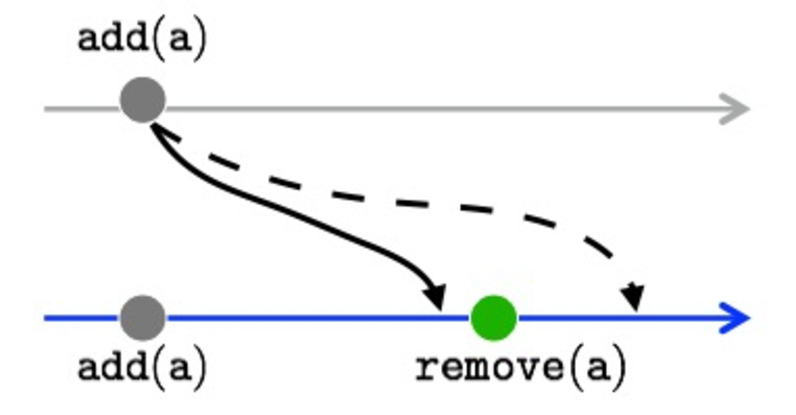
\includegraphics[width=0.30 \textwidth]{./figures/OR-Set-simple}
  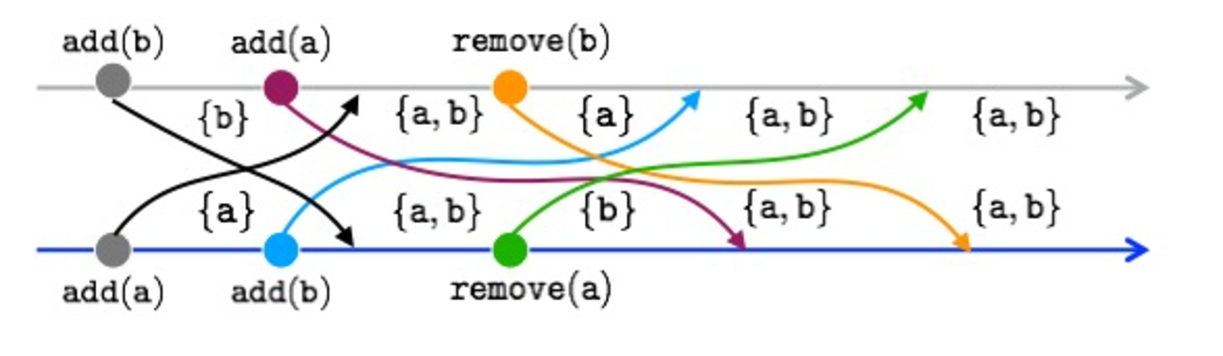
\includegraphics[width=0.70 \textwidth]{./figures/OR-Set-weird}
  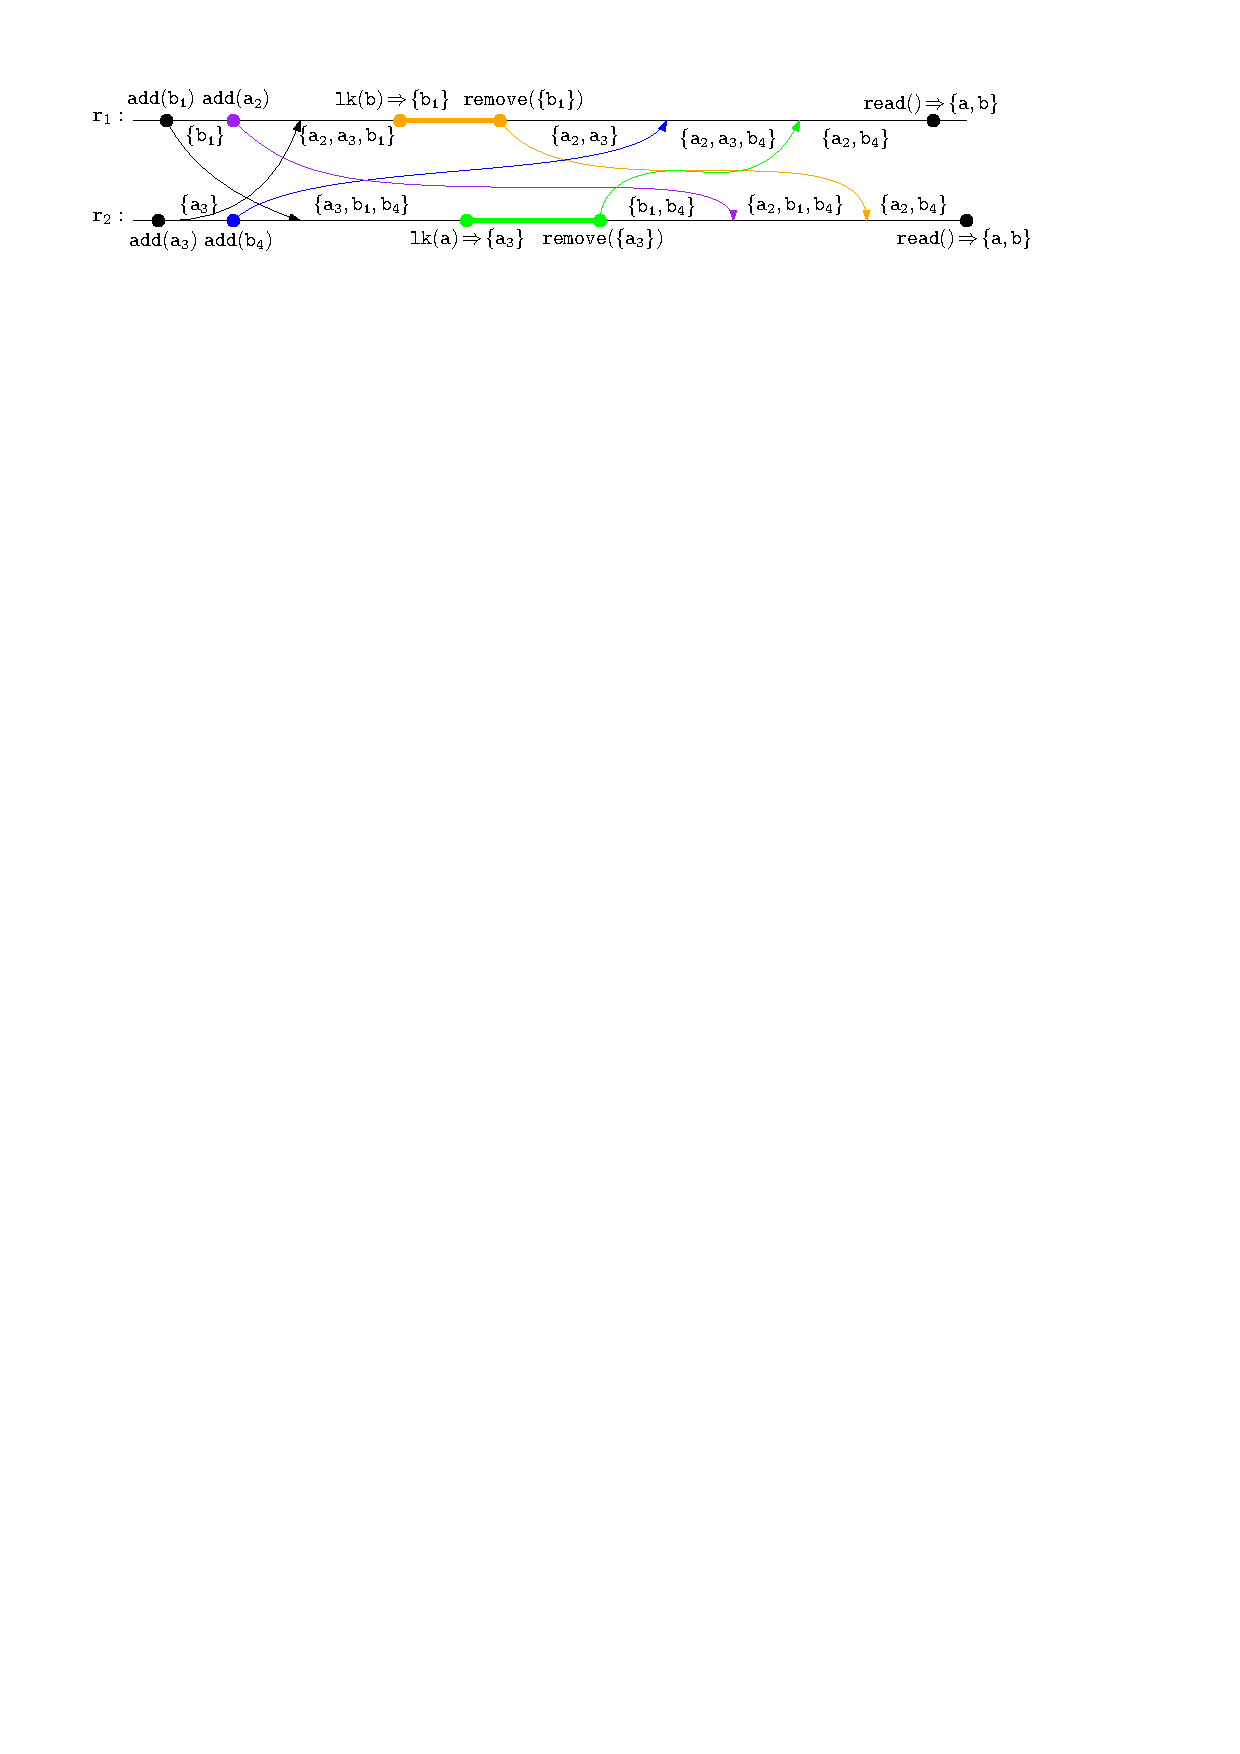
\includegraphics[width=0.90 \textwidth]{./figures/OR-Set-lk-rem}
  \caption{OR-Set non-linearizable execution.}
  \label{fig:or-set-not-lin}
\end{figure}

For our definition of \CRDTLinshort{} we will distinguish between
\emph{update} and \emph{query} operations.
%
We will impose two constraints, one on updates and the other on
queries:
\begin{itemize}
\item For updates we require that there exists a total order of all
  the updates in the execution -- essentially a linearization -- such
  that the resulting state of the object -- or any intermediate state --
  can be explained by executing the \emph{specification} of these
  updates in order.
%
  Essentially, reachable states of the implementation are related to
  specification states that can be reached by a certain linearization of
  the updates.
%
  \gpnote{Example?}
\item Unfortunately, this simple requirement does not suffice for
  query operations, since the system model allows for updates to arrive
  to different replicas in different order.
%
  Hence, for \CRDTLinshort{} we will require that the result of any
  query can be explained by consider a \emph{sub-sequence} of the above
  mentioned global linearization up updates.
\end{itemize}
This definition will be made precise in~\autoref{sec:distributed-lin}.

\gpnote{Maybe add a read example first?}
Coming back to our OR-Set example in~\autoref{fig:or-set-not-lin}, we
have that the \lstinline|remove| operation behaves as both a query
(observing a certain number of updates on the element to be removed)
and an update (by removing said updates).
%
To cope with such cases, we will consider in our definition that
query-update operations can be split into a query part, which only
reads the state -- and hence can see only a sub-sequence of the
linearization of updates --, and an update part which will use the
results of the prior query.
%
For instance, \lstinline|remove| will be split into a query part where
only the elements that are visible at the time of the remove are
selected, and an update part where only those elements selected are
erased.
%
Evidently, this requires some mechanism for ``marking'' the adds that
are concerned.
%
We will consider that each add has a unique identifier.
%
Then, the query part of a remove returns a set of unique identifiers
to be removed.
%
Any identifier not in this set will remain in the set after the update
part of the remove.
%
The second part of~\autoref{fig:or-set-not-lin} shows this rewriting
where we denote by \lstinline|lk| (for lookup) the query part of
remove, which returns a set of elements to be removed, and a
\lstinline|remove| operation taking a set of elements to be removed.
%
In this case, our definition of linearizability is just as before.
%
To linearize this execution, when contemplating only the updates, we
can chose any order consistent with the order in which operations are
performed in each replica and the result is consistent with the
specification of a set.
%
We discuss the details of this constructions in the next section.


% Method $\mathit{add}(a,b)$ intends to add item $a$ into the list at a
% position immediately after that of a existing item $b$. Method
% $\mathit{rem}(a)$ removes $a$ from the list. Method $\mathit{read}$
% returns the current list content. When the current replica does
% $\mathit{add}(a,b)$, it generate a tuple $(a,ts_a,ts_b)$ and put it
% into $N$. Here $ts_b$ is the time-stamp of $b$, and $ts_a$ is a new
% time-stamp that is larger than any time stamp in $N$. When the current
% replica does $\mathit{rem}(a)$, it put $a$ into tombstone. When the
% current replica does $\mathit{read}$, it uses function
% $\mathit{trans}(N,\mathit{Tomb})$ to return the list seen by the
% current replica, which is a sequences obtained by traversing $N$ in
% prefix order (children are visited in decreasing time-stamp order) and
% keeping only items that are not in $\mathit{Tomb}$.

%      precondition : %@|$\exists$|@ k. (a,k) @|$\in$|@ S
%let @|$\alabel = \alabellongind[remove]{a,R}{\bot}{i}$|@
%      //@ @|$\alpha(S) \xrightarrow{\alabelshort[add]{a,k}} \alpha(S')$|@
%       //@ @|$\alpha(S) \xrightarrow{\alabellongind[readIds]{a}{R}{}} \alpha(S)$|@
%       //@ @|$\alpha(S) \xrightarrow{\alabelshort[remove]{a,R}} \alpha(S')$|@
%     //@ @|$\alpha(S) \xrightarrow{\alabellongind[read]{}{A}{}} \alpha(S)$|@

% In the downstream of a $\alabellongNoret[\mathit{add}]{\argv}$
% operation, an tuple $(\argv,\ats)$ will be added to the local state;
% while in the downstream of a $\alabellongNoret[\mathit{add}]{\argv}$
% operation, a set $S_1$ will be removed from the local state. We call
% such tuple $(\argv,\ats)$ or set $S_1$ the content of the downstream.
% The following is the condition $C_2$ for or-set implementati.

%%% Local Variables:
%%% mode: latex
%%% TeX-master: "draft"
%%% End:
